\section{Single Phase Half Wave Controlled Rectifier with RL load}

\subsection{Circuit used for simulation}

% figure that is centered on the page
\begin{figure}[h]
    \centering
    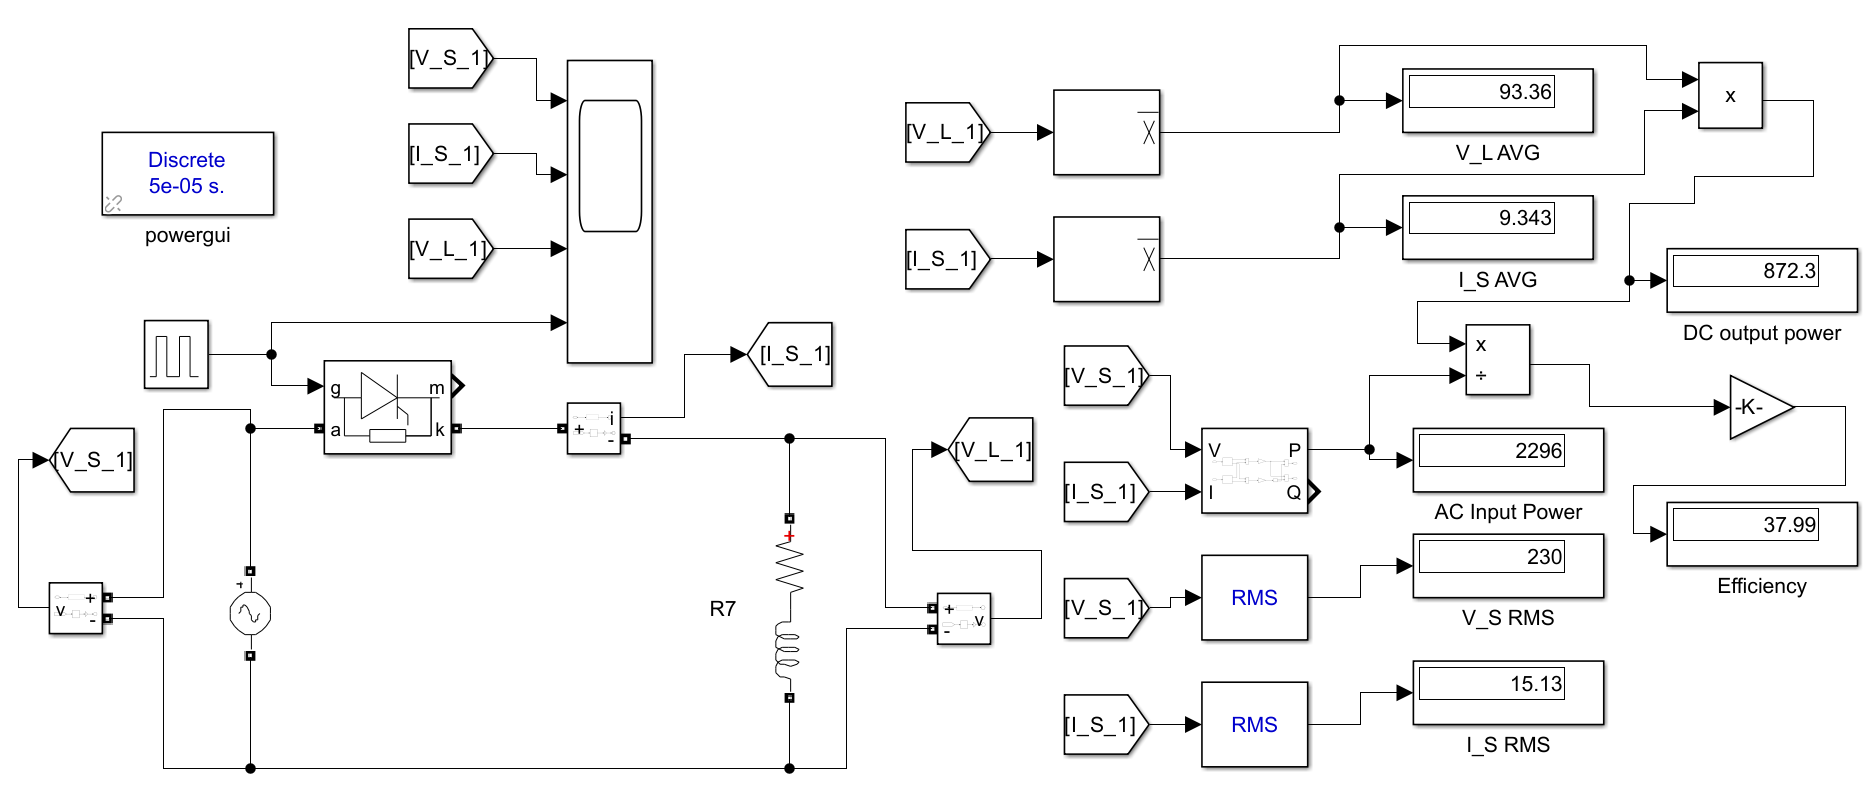
\includegraphics[width=1.0\textwidth]{images/experiment-1/circuit-diagram-experiment-06.png}
    \caption{Circuit for Single Phase Half Wave Controlled Rectifier with RL load  (Firing Angle = 30$ ^\circ $)}
    \label{Fig_simulation_circuit_single-phase-half-wave-controlled-rectifier-with-RL-load}
\end{figure}

\subsection{Components Required}

\begin{table}[h]
    \renewcommand{\arraystretch}{1.3}
    \label{table_components_required_single-phase-half-wave-controlled-rectifier-with-RL-load}
    \centering
    \begin{tabular}{|c|c|c|c|}
        \hline
        Sr. No & Parameters                     & Ratings            & Quantity \\
        \hline
        \hline
        1      & AC Single Phase Voltage Source & 230V ($ V_{rms} $) & 1        \\
        \hline
        2      & Resistor                       & 10$ \Omega $       & 1        \\
        \hline
        3      & Inductor                       & 10mH               & 1        \\
        \hline
        4      & Diode                          & -                  & 1        \\
        \hline
        5      & Voltmeter                      & -                  & 2        \\
        \hline
        6      & Ammeter                        & -                  & 1        \\
        \hline
        7      & Thyristor                      & -                  & 1        \\
        \hline
    \end{tabular}
    \caption{Components for Single Phase Half Wave Controlled Rectifier with RL load}

\end{table}




\subsection{Observations}

\begin{table}[h]
    \renewcommand{\arraystretch}{1.3}
    \label{table_observation_single-phase-half-wave-controlled-rectifier-with-RL-load}
    \centering
    \begin{tabular}{|c|c|c|}
        \hline
        Parameters                              & Theoretical Values & Simulation Values \\
        \hline
        \hline
        AC Input Voltage ($ V_{in,rms} $)       & 230V               & 230V              \\
        \hline
        Output Average Voltage ($ V_{o,avg} $)  & 96.6V              & 93.36V            \\
        \hline
        Output Average Current ($ I_{o,avg}  $) & 9.66A              & 9.343A            \\
        \hline
    \end{tabular}
    \caption{Observations for Single Phase Half Wave Controlled Rectifier with RL load}

\end{table}


Upon providing the firing gate pulse to the thyristor, it is observed that the circuit begins conducting. Due to the presence of an inductive component in the load, the output current lags behind the output voltage, leading to the conduction of the diode until the output current approaches zero. Consequently, the output voltage becomes negative during this duration. After the output current falls to zero, the thyristor ceases conduction, and the output voltage returns to zero as well.
Additionally, the DC output power was estimated to be 872.3W, while the AC input power was found to be 2296W, resulting in an overall efficiency of 37.99\%.



% \pagebreak

\subsection{Resultant Waveforms}

% figure that is centered on the page
\begin{figure}[h]
    \centering
    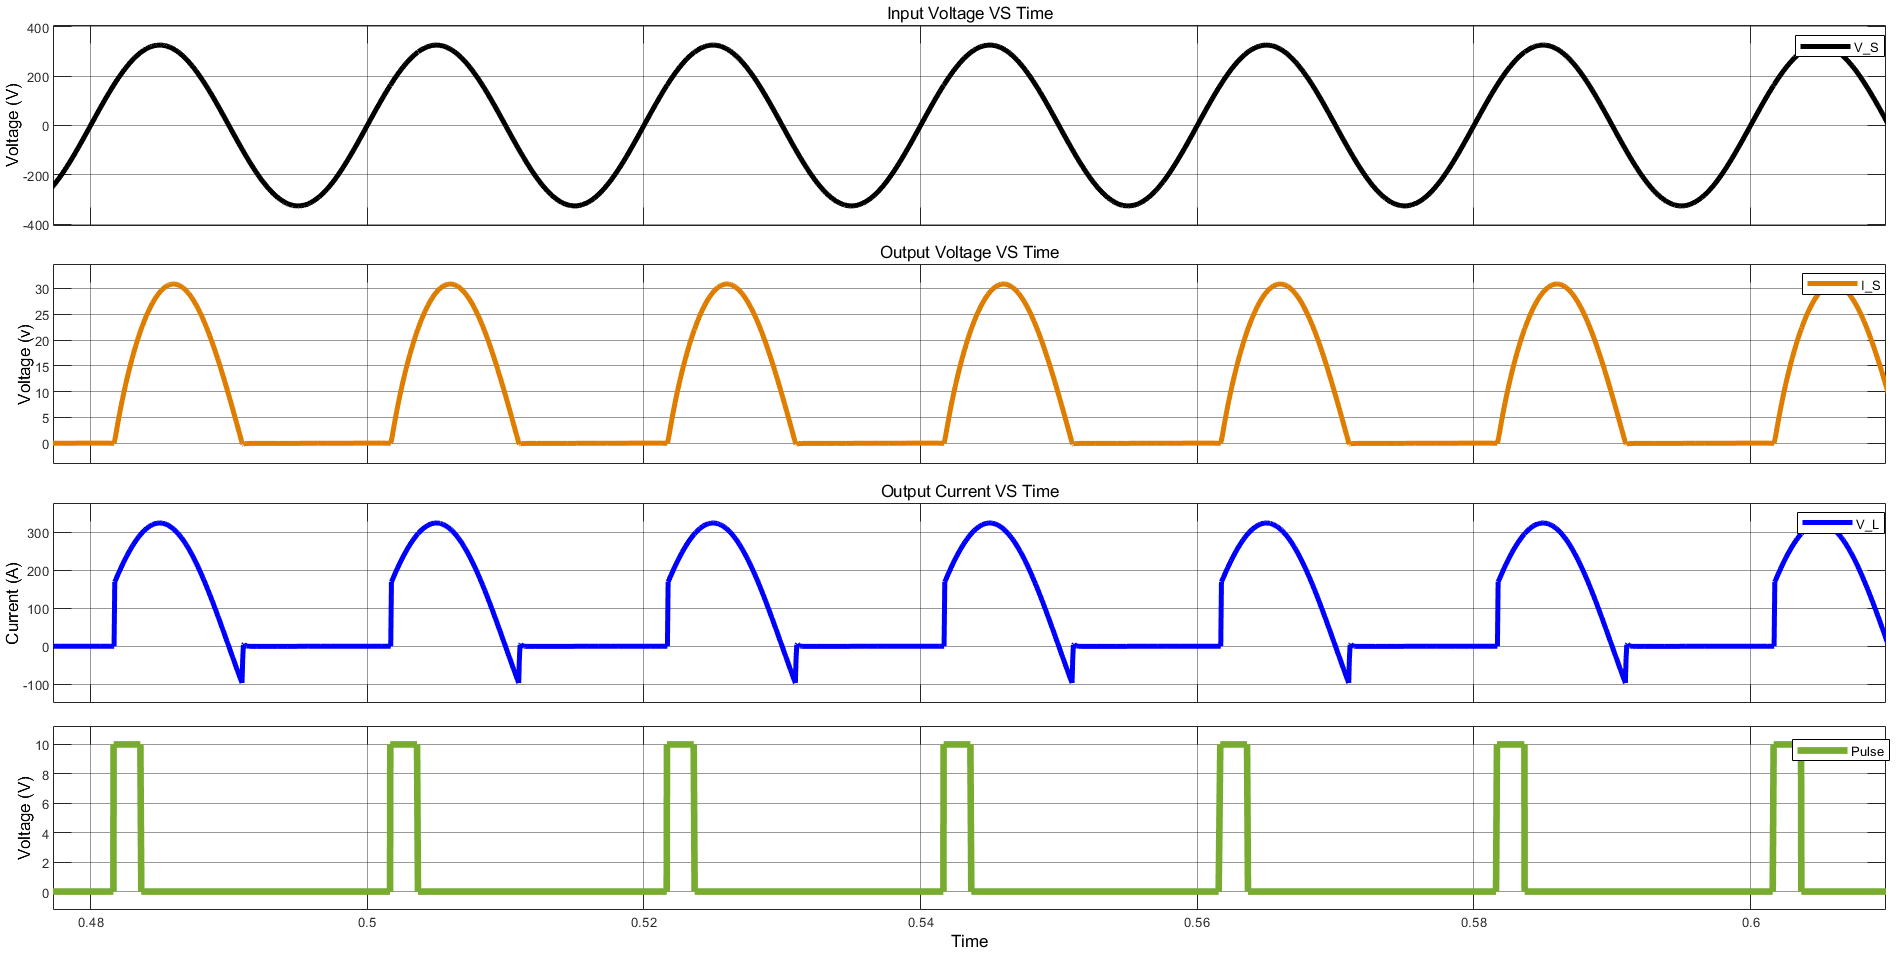
\includegraphics[width=1\textwidth]{images/experiment-1/circuit-scope-experiment-06.png}
    \caption{Scope Waveforms for Single Phase Half Wave Controlled Rectifier with RL load}
    \label{Fig_waveform_single-phase-half-wave-controlled-rectifier-with-RL-load}
\end{figure}

\pagebreak
